\section{Introduction}

When reading a scientific article, the reader's comprehension of the text may
be greatly improved by inclusion of charts, tables and figures that help summarise information.
For example, in \figref{table-explanation}, information about climate change models
has been summarized in a table, with the supporting paragraph providing the reader
with an interpretation of the information in the table, references to ``SSP-'' within
the text mean the rows of the table, with the qualification that the columns all refer
to data about the 21st century.

Visualizations -- tables included -- abstract and summarize data, in order to make
it easier for the reader to understand, but the readers comprehension can be aided
further by building interactive features into the visualization. Allowing the user
to, for example, click on parts of a chart to see what data it summarizes allows
them to get a better sense of how the data was used, and what the author is trying
to say. By making the text itself an interactive feature, the readers understanding
can be improved yet again.

Authoring of such articles is difficult and time-consuming, and taking an article
and building interactive features into its visualisations requires a further investment
of effort, often on an ad-hoc basis. As yet, there has been no tool that extends
interactivity features to treat text as an interactive visual element. It is not
entirely clear what such features look like when extended to text, and requiring
the author to spend even more time effectively programming their article imposes
a significant burden on the author. 

Some of the difficulty can be mitigated by building visualizations in a language
which provides automatic support for interaction, but these do not provide tools
or support for linking data directly to the text of an article. An article will
be full of references to items of discourse, and asking the author to manually
link each reference to its referent for the purposes of interaction is liable to
error, or the user simply giving up. An automated tool is required. 

\begin{figure}
   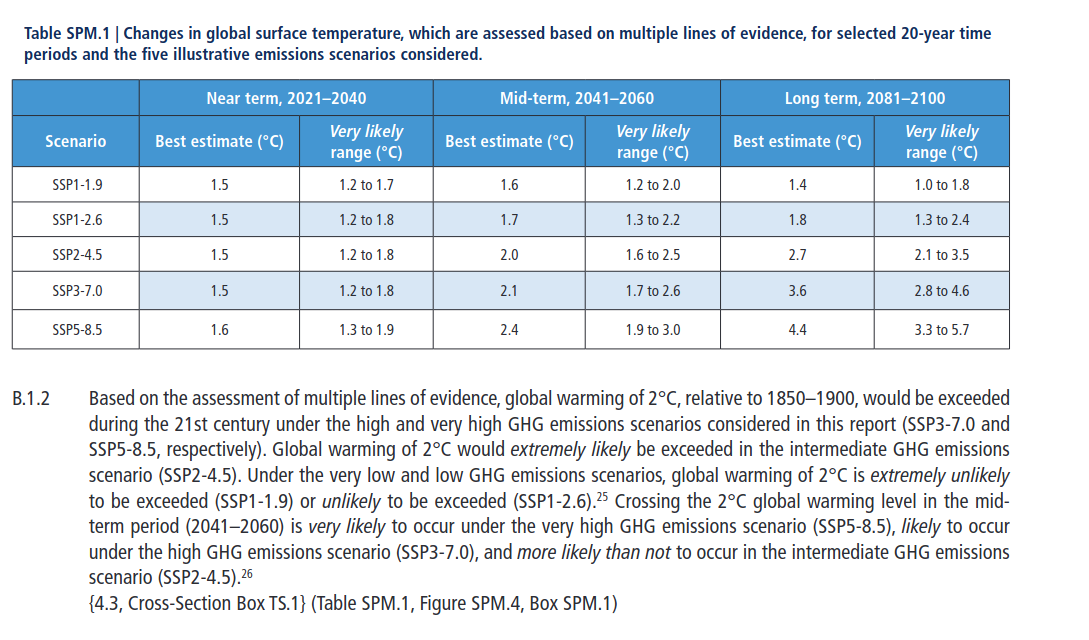
\includegraphics[width=0.9\textwidth]{fig/ipcc-table-explanation.png}
   \caption{Explanation based on the contents of a table}
   \label{fig:table-explanation}
\end{figure}